%!TEX root = ./aistats_2019_sketchmcmc_supp.tex


% \section{Visual Comparison with Existing Approaches}

% In this section, we provide the results presented in \cite{deshpande2018generative} for visual comparison. These results are obtained by running different IGM approaches on the MNIST dataset, namely GAN \cite{goodfellow2014generative}, Wasserstein GAN (W-GAN) \cite{arjovsky2017wasserstein} and the Sliced-Wasserstein Generator (SWG) \cite{deshpande2018generative}.

% \begin{figure}[h!]
% \centering
% 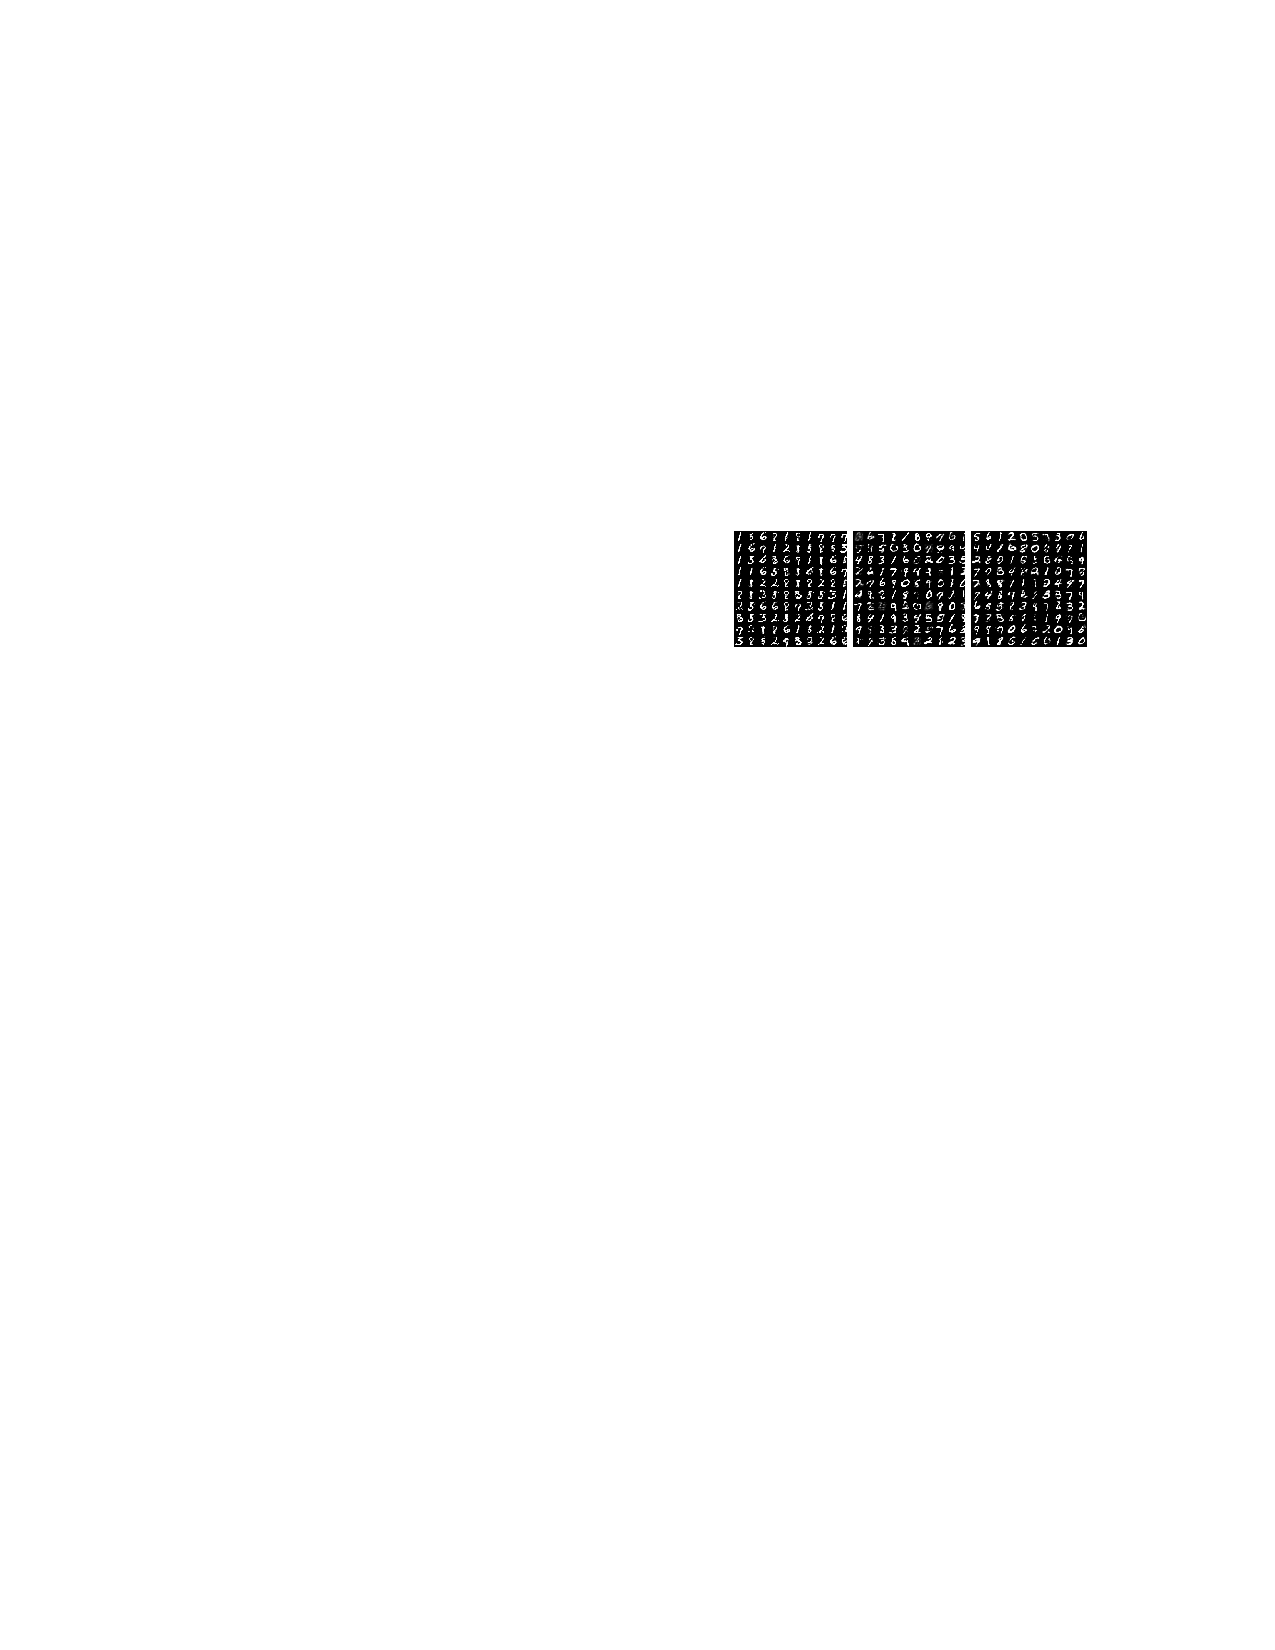
\includegraphics[width=0.5\columnwidth]{mnist_all.pdf}
% \caption{Performance of GAN (left), W-GAN (middle), SWG (right) on MNIST. (The figure is directly taken from \cite{deshpande2018generative}.) }
% \label{fig:mnistall}
% \end{figure}


\section{Additional Experimental Results}

\subsection{Implementation details}

\paragraph{The Sliced Wasserstein Flow}
The whole code for the Sliced Wasserstein Flow was implemented in Python, for use with Pytorch\footnote{\url{www.pytorch.org}.}. The code was written so as to run efficiently on GPU, and is available on the publicly available repository related to this paper\footnote{\url{github.com/removed_for_double_blind}.}.

In practice, the SWF involves relatively simple operations, the most important being:
\begin{itemize}
  \item For each random $\theta\in\{\theta_n\}_{n=1\dots N_\theta}$,  compute its inner product with all items from a dataset and obtain the empirical quantiles for these \emph{projections}.
  \item At each step $k$ of the SWF, for each projection $z=\left<\theta, \bar{X}^i_k\right>$, apply two piece-wise linear functions, corresponding to the scalar optimal transport $\psi_{k, \theta}'(z)$.
\end{itemize}
Even if such steps are conceptually simple, the quantile and required linear interpolation functions were not available on GPU for any framework we could figure out at the time of writing this paper. Hence, we implemented them ourselves for use with Pytorch, and the interested reader will find them in the Github repository dedicated to this paper.

Given these operations, putting a SWF implementation together is straightforward, and the online code is able to apply it on any dataset.

\paragraph{Vanilla autoencoders for reducing data dimension}

As mentioned in the text, we used autoencoders to reduce the dimensionality of the transport problem. The structure of these networks is the following:

\begin{itemize}
  \item $\textbf{Encoder}$ Four 2d convolution layers with \(num_chan_out, kernel size, stride, padding\) being $(3,3,1,1)$, $(32,2,2,0)$, $(32,3,1,1)$, $(32, 3,1,1)$, each one followed by a relu activation. At the output, a linear layer gets the desired bottleneck size.

  \item $\textbf{Decoder}$ A linear layer gets from the bottleneck features to a vector of dimension $8192$, which is reshaped as $(32, 16,16)$. Then, three convolution layers are applied, all with $32$ output channels and \(kernel size, stride, panning\) being respectively $(3,1,1)$, $(3,1,1)$, $(2,2,0)$. A 2d convolution layer is then applied with an output number of channels being that of the data \($1$ for black and white, $3$ for colour\), and a \(kernel size, stride, panning\) as $(3,1,1)$. In any case, all layers are followed by a relu activation, and a sigmoid activation is applied a the very output.
\end{itemize}

Once these networks defined, these autoencoders are trained in a very simple manner by minimizing the squared differenc between input and output over the training set of the considered dataset (here MNIST or FashionMNIST). This training was achieved with the Adam algorithm \cite{kingma2014adam} with learning rate $1e-3$.

No additional training trick was involved as in Variational Autoencoder \cite{kingma2013VAE} to make sure the distribution of the bottleneck features match some prior. The core advantage of the proposed method in this respect is indeed to turn any previously learned AE as a generative model, by automatically and non-parameterically transporting particles drawn from an arbitrary prior distribution $\mu$ to the observed empirical distribution $\nu$ of the bottleneck features over the training set.

\subsection{Additional results}

In Figures~\ref{fig:suppmnist} and \ref{fig:suppfmnist} below, we provide the evolution of the SWF algorithm on the Fashion MNIST and the MNIST datasets in higher resolution.

\newcommand{\picwidth}{0.15}%originally 0.24

\begin{figure}
\centering
\includegraphics[width=\picwidth\columnwidth]{supplementary/mnist/train_image_0.png}
\includegraphics[width=\picwidth\columnwidth]{supplementary/mnist/train_image_10.png}
\includegraphics[width=\picwidth\columnwidth]{supplementary/mnist/train_image_20.png}
\includegraphics[width=\picwidth\columnwidth]{supplementary/mnist/train_image_30.png}\\
\includegraphics[width=\picwidth\columnwidth]{supplementary/mnist/train_image_40.png}
\includegraphics[width=\picwidth\columnwidth]{supplementary/mnist/train_image_50.png}

\includegraphics[width=\picwidth\columnwidth]{supplementary/mnist/train_image_100.png}
\includegraphics[width=\picwidth\columnwidth]{supplementary/mnist/train_image_200.png}
\caption{The evolution of SWF through 200 iterations on the MNIST dataset. Plots are for $1$, $11$, $21$, $31$, $41$, $51$, $101$ and $201$ iterations}
\label{fig:suppmnist}
\end{figure}

\begin{figure}
\centering
\includegraphics[width=\picwidth\columnwidth]{supplementary/alternative_fmnist/train_image_0.png}
\includegraphics[width=\picwidth\columnwidth]{supplementary/alternative_fmnist/train_image_10.png}
\includegraphics[width=\picwidth\columnwidth]{supplementary/alternative_fmnist/train_image_20.png}
\includegraphics[width=\picwidth\columnwidth]{supplementary/alternative_fmnist/train_image_30.png}\\
\includegraphics[width=\picwidth\columnwidth]{supplementary/alternative_fmnist/train_image_40.png}
\includegraphics[width=\picwidth\columnwidth]{supplementary/alternative_fmnist/train_image_50.png}

\includegraphics[width=\picwidth\columnwidth]{supplementary/alternative_fmnist/train_image_100.png}
\includegraphics[width=\picwidth\columnwidth]{supplementary/alternative_fmnist/train_image_200.png}
\caption{The evolution of SWF through 200 iterations on the FashionMNIST dataset. Plots are for $1$, $11$, $21$, $31$, $41$, $51$, $101$ and $201$ iterations}
\label{fig:suppfmnist}
\end{figure}







% \section{Details of Computing $(F_{\theta_{n}^*\#\hat{\mu}}^{-1} \circ F_{\theta^*_{n}\#\nu}) $}


% \umut{Antoine. -- sorting, interpolation etc}

% \begin{figure}
% \begin{centering}
% \setlength\tabcolsep{1pt}
% \begin{tabular}{cccccc}
% $\lambda=0$ & $\lambda=0.1$ & $\lambda=0.2$ & $\lambda=0.3$ & $\lambda=0.5$ & $\lambda=1$\tabularnewline
% 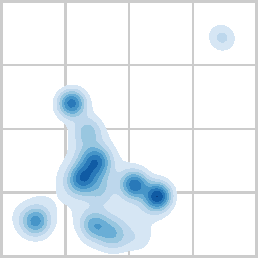
\includegraphics[width=2cm]{figures/supplementary/regularization/r0_output_dist_k=70-crop.pdf} & 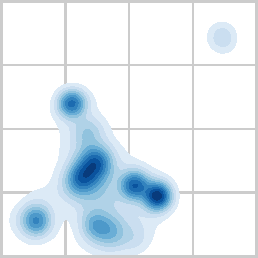
\includegraphics[width=2cm]{figures/supplementary/regularization/r01_output_dist_k=70-crop.pdf} & 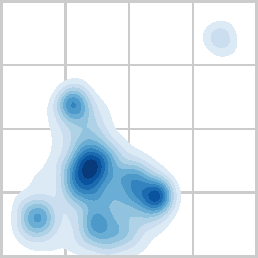
\includegraphics[width=2cm]{figures/supplementary/regularization/r02_output_dist_k=70-crop.pdf} &  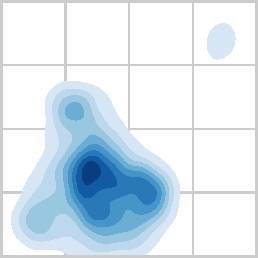
\includegraphics[width=2cm]{figures/supplementary/regularization/r03_output_dist_k=70-crop.pdf}&  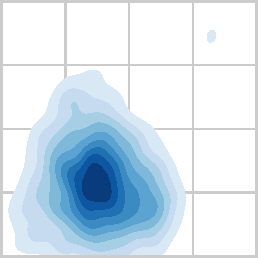
\includegraphics[width=2cm]{figures/supplementary/regularization/r05_output_dist_k=70-crop.pdf} &  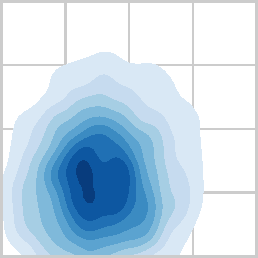
\includegraphics[width=2cm]{figures/supplementary/regularization/r1_output_dist_k=70-crop.pdf}
% \end{tabular}
% \par\end{centering}
% \caption{Influence of the regularization parameter $\lambda$. The higher $\lambda$, the more entropic the output distribution.\label{fig:lambda_supp}}
% \end{figure}
